\subsection{Methods of Elenchus}

The name ``elenchus'' comes from the Greek word ``elenchein,'' which means to examine. 
The method of elenchus is often seen as a form of cross-examination \cite{Cross-Examination2021,WinArgument2006}, in which a teacher uses questions and counter-questions to expose contradictions and inconsistencies in a student's beliefs and attitudes, in order to arrive at a deeper understanding of a topic.

An example of the method of elenchus in action would be a dialogue between Socrates and a student in which Socrates asks a series of questions to help the student understand the concept of justice. For example, Socrates might ask the student to define justice, and then ask follow-up questions to expose any contradictions or inconsistencies in the student's definition. Through this process of questioning and counter-questioning, Socrates aims to help the student arrive at a deeper understanding of justice.

\begin{comment}
How do we design a prompt template for these methods?
When utilizing these methods in a dialogue with a language model, the primary focus is on identifying and addressing inconsistencies. This can be done by following a process similar to legal cross-examination, first establishing the credibility of the language model's sources, identifying and addressing inconsistencies of multiple sources (witnesses), and highlighting key points that support the conclusions \cite{}.

It is important to note that a language model can produce biased or incorrect answers. To ensure the credibility of the answers, it can be helpful to ask the language model for its sources of information and then validate the credibility of those sources. By having multiple answers, their information sources, and the credibility of those sources, a more trustworthy answer can be derived.
\end{comment}

\begin{table}[htbp!]
\caption{Identifying Inconsistency (ChatGPT 1/23/2023)}
\label{tab-lake}
%\resizebox{\textwidth}{!}
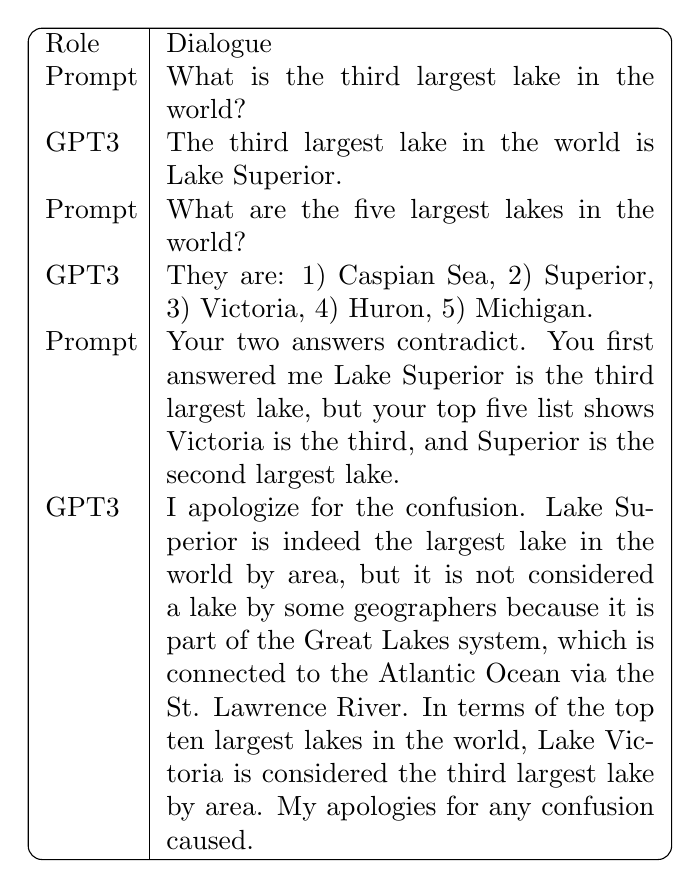
\begin{tikzpicture}
\begin{normalsize}
\node (table) [inner sep=0pt] {
\begin{tabular}{p{1.1cm}|p{6.2cm}}
\toprule
Role & Dialogue \\
\midrule
Prompt & {What is the third largest lake in the world?} \\
GPT3 & {The third largest lake in the world is Lake Superior. } \\
Prompt & {What are the five largest lakes in the world?} \\
GPT3 & {They are:
1) Caspian Sea, 2) Superior, 3) Victoria,
4) Huron, 5) Michigan.
} \\
Prompt & {Your two answers contradict. You first answered me Lake Superior is the third largest lake, but your top five list shows Victoria is the third, and Superior is the second largest lake.} \\
GPT3 & {I apologize for the confusion. Lake Superior is indeed the largest lake in the world by area, but it is not considered a lake by some geographers because it is part of the Great Lakes system, which is connected to the Atlantic Ocean via the St. Lawrence River. In terms of the top ten largest lakes in the world, Lake Victoria is considered the third largest lake by area. My apologies for any confusion caused.} \\
%\bottomrule
\end{tabular}
};
\draw [rounded corners=.5em] (table.north west) rectangle (table.south east);
\end{normalsize}
\end{tikzpicture}
\vspace{-.1in}
\end{table}
\hfill \break
\noindent
{\bf Example}: {\em What is the third largest lake in the world?}
%\subsubsection*{Example: What is the third largest lake in the world?}
\hfill \break
Figure~\ref{tab-lake} presents an example prompting session with ChatGPT.  The first prompt queries ChatGPT for the third largest lake in the world.  ChatGPT returns ``Lake Superior.''  The second prompt asks for the ten largest lakes, on which the thrid largest is ``Lake Victoria.''  After pointing out the inconsistency to ChatGPT, it returns that ``Lake Victoria'' is the right answer to the first prompt, and it also provides the reason for its mistake.
(We tested on ``the fifth highest mountain in the world'' and went through a similar consistency check, and the answer provided by ChatGPT is accurate.)

%Depending on the importance of the answer, a prompt template may want to identify three or more reliable sources and then query LLMs for both answers and references. A credential check on references is similar to a credential check on a witness in a legal proceeding. 
